\documentclass[12pt]{article}
\usepackage[margin=1in]{geometry}% Change the margins here if you wish.
\setlength{\parindent}{0pt} % This is the set the indent length for new paragraphs, change if you want.
\setlength{\parskip}{5pt} % This sets the distance between paragraphs, which will be used anytime you have a blank line in your LaTeX code.
% \pagenumbering{gobble}% This means the page will not be numbered. You can comment it out if you like page numbers.

\usepackage{amsmath,amsthm,amssymb} % These packages allow the most of the common "mathly things"
\usepackage{graphicx} % This package allows you to add images.
\usepackage{float}
\usepackage{biblatex}
\usepackage{hyperref}

\begin{filecontents}{\jobname.bib}
@book{Stevens2003,
    Author = {Brian L. Stevens and Frank L. Lewis and Eric N. Johnson},
    Publisher = {Wiley},
    Title = {Aircraft Control and Simulation},
    Year = {2003}}

@article{Wharington1993,
    Author = {John M. Wharington and Philip W. Blythe and Israel Herszberg},
    Title = {The Development of Neural Network Techniques for the System Identification of Aircraft Dynamics},
    Publisher = {5th Australian Aeronautical Conference},
    Adress = {Melbourne},
    Year = {1993}}
}
\end{filecontents}

\addbibresource{\jobname.bib}

\title{System Identification of Aircraft Dynamics Using Neural Networks}
\author{Fidel Echevarria Corrales}
\date{\today}

\begin{document}

\maketitle

The proposed work consists on the development of a tool capable of estimating aircraft aerodynamic derivatives, with flight dynamic states history as only input. In the subsequent section the dynamic model will be defined and detailed.

% \clearpage

\section{Dynamic Model Definition}

\subsection{Model definition and sign convention}

Vehicle dynamics are modelled by taking into account forces and moments \cite{Stevens2003}.

\begin{equation}\label{eq1}
    q=\frac{1}{2} \cdot \rho \cdot V^2
\end{equation}

\begin{equation}\label{eq2}
\begin{gathered}
    L=q \cdot S \cdot C_L \\
    D=q \cdot S \cdot C_D \\
    Y=q \cdot S \cdot C_Y
\end{gathered}
\end{equation}

\begin{equation}\label{eq2}
\begin{gathered}
    l=q \cdot S \cdot b \cdot C_l \\
    m=q \cdot S \cdot c \cdot C_m \\
    n=q \cdot S \cdot b \cdot C_n
\end{gathered}
\end{equation}

\begin{equation}\label{eq2}
\begin{gathered}
    C_L=C_{L_0} + C_{L_{\alpha}} \cdot \alpha \\
    C_D=C_{D_0} + K \cdot {C_L}^2 + C_{D_{\beta}} \cdot \beta \\
    C_Y=C_{Y_{\beta}} \cdot \beta + C_{Y_{\delta r}} \cdot \delta r
\end{gathered}
\end{equation}

\begin{equation}\label{eq2}
\begin{gathered}
    C_l=C_{l_{\beta}} \cdot \beta + C_{l_{\delta a}} \cdot \delta a + C_{l_{\delta r}} \cdot \delta r + \frac{b}{2V} \cdot (C_{l_p} \cdot p + C_{l_r} \cdot r) \\
    C_m=C_{m_0} + C_{m_{\alpha}} \cdot \alpha + C_{m_{\delta e}} \cdot \delta e + \frac{c}{2V} \cdot (C_{m_q} \cdot q + C_{m_{\dot{\alpha}}} \cdot \dot{\alpha}) \\
    C_n=C_{n_{\beta}} \cdot \beta + C_{n_{\delta a}} \cdot \delta a + C_{n_{\delta r}} \cdot \delta r + \frac{b}{2V} \cdot (C_{n_p} \cdot p + C_{n_r} \cdot r)
\end{gathered}
\end{equation}

\setcounter{figure}{0}
\begin{figure}[H]
\centering
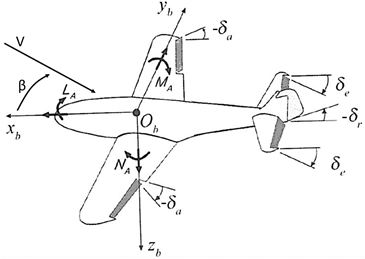
\includegraphics[width = .6\textwidth]{signs}
\label{fig:A.1}
\caption{Coordinate axes definition}
\end{figure}

\subsection{Glossary}

$\rho \equiv$ Air density

$q \equiv$ Dynamic pressure

$S \equiv$ Wing reference surface

$b \equiv$ Wingspan

$c \equiv$ Mean chord

$(L, D, Y) \equiv$ Aerodynamic forces in axes $(-x, y, -z)$. Lift, Drag, Sideforce

$(C_L, C_D, C_Y) \equiv$ Aerodynamic force coefficients

$(l, m, n) \equiv$ Aerodynamic moments in body-axes

$(C_l, C_m, C_n) \equiv$ Aerodynamic moment coefficients

$(\delta_a, \delta_e, \delta_r) \equiv$ Control surface deflections (ailerons, elevator, rudder)

$(p, q, r) \equiv$ Angular velocities in body axes

$\alpha \equiv$ Angle of attack

$\dot{\alpha} \equiv$ Derivative of angle of attack with respect to time

$\beta \equiv$ Sideslip angle \newline

Aerodynamic derivative $C_{x_y}$ provides information about the effect on the variable $x$ caused by a unitary increment in the variable $y$.

\section{Objective}

The presented dynamic model will be used to propagate the kinematic states of the aircraft iteratively, taking into account other forces such as gravity or engine thrust. The control inputs are the aerodynamic control surfaces (elevator, ailerons and rudder). The objective is to develop a tool which takes as input the history of flight states of an aircraft and estimates a set of aerodynamic coefficients using a pre-trained neural network. Lastly, a simulator with the original aircraft dynamics will be automatically generated. The neural network will be trained by generating dynamic state history datasets using a simulator which randomly varies aerodynamic coefficients generating aircraft models, and labels each flight dataset with its corresponding true set of aerodynamic derivatives. In a first approach, each training sample will be composed of the history of several state variables, including control surface deflections, forces (without gravity), moments, linear velocities and angular velocities.

\setcounter{figure}{1}
\begin{figure}[H]
\centering
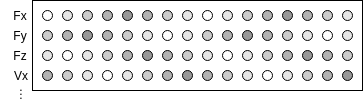
\includegraphics[width = .6\textwidth]{diagram}
\label{fig:A.2}
\caption{State history training sample}
\end{figure}

For the training phase, it will be really important to replicate the chaotic nature of turbulences. This is necessary so that the network doesn’t specialize in the ideal dynamic flight generated by the training simulator, and thus is capable of generalizing well with real flight data once it has been trained. Additionally, aircraft command history needs to have a random component, given that real flight data control history will never be the same. In order to be able to generate somewhat realistic random trajectories for training, an adaptive inverse-based control algorithm will be implemented to act as a control augmentation system for each randomly generated training sample. This way, instead of randomizing the direct control surface inputs, other higher level variables may be randomly commanded (pitch and roll commands). This also decreases the probability of the randomly generated control inputs producing a divergence in the simulation. An additional difficulty is that some aircraft derivative sets will produce an uncontrollable system, causing the simulator to eventually diverge. These cases will be discarded, taking only as valid those sets of random derivatives which have generated a controllable system.

Research and analysis will be carried out in order to determine the best possible neural network architecture for this project. In a first glance, bidimensional convolutional neural networks, as well as LSTM networks, both seem to be suitable candidates. The application will be developed using \href{https://www.python.org/}{Python} programming language, together with \href{https://www.tensorflow.org/}{TensorFlow} (and \href{https://www.tensorflow.org/guide/keras}{Keras}) libraries for the neural network development and deployment. Open-source software program \href{https://www.flightgear.org/}{FlightGear} will be used as a graphical engine for the aircraft simulator.

The concept of neural network techniques for system identification of aircraft dynamics has been previously investigated for feasability and to identify associated advantages and disadvantages, with very promising conclusions \cite{Wharington1993}.

\printbibliography

\end{document}